% CREATED BY MAGNUS GUSTAVER, 2020
\chapter{Theory}
% Kan skriva ut den här när vi har skrivit fler delar av detta kapitel
This chapter covers the theory and common problems of modern programming languages blah blah blah.

% Behöver verkligen inte vara den första sectionen utav kapitlet
% Jag antar här att teori ska va presens som introduktion
\section{Memory management}
Memory is a fundamental and finite resource that allows computers to store data which leads to the possibility
of executing programs that have to be loaded into memory. Programs need memory to store data such as variables
and objects in memory during execution. Due to memory being a finite resource, its amount limits the size and
the capabilities of an executing program. Since a computer's memory is shared across multiple programs
executing concurrently, it is important that one single program does not try to allocate or use all of the
available memory, resulting in limitations on the rest of the system and executing programs. Therefore
it is of great importance to minimize the amount of memory allocated to or by a program, without
interfering with its execution.\\

In modern high-level programming languages such as Java and Haskell, memory is automatically managed by
their runtimes (code that is executed during the program's execution which enables the program to interact
with system resources). Depending on the use case of the language, the runtime varies in size. For example, lower-level
languages such as C have very small runtimes since the language is already close to using system resources like
memory, close meaning that a developer in this language can directly request resources from the system
without the use of the language runtime. In high-level languages system resources are allocated by
the runtime, where the runtime can efficiently keep track of used and unused but allocated memory.
Algorithms for freeing up memory can then be applied by the runtime on this data to minimize the amount
of memory used by the program. This process of freeing up memory is also well-known as garbage collection.\\

\subsection{Memory layout and program interaction}

For a program to be executed it has to be compiled and then loaded into memory by the operating system.
The compiled program is split into smaller segments called stack, heap, text, bss, and data [insert source].
The stack segment contains the call stack of the program, which is used for function calls, saving registers,
and storing local variables. The bss and data segments are of less importance and are used for storing
global variables in the program, uninitialized and initialized respectively. The text segment
contains the program code in byte-code format used by the central processing unit (CPU) to execute the
compiled program. The most important segment for memory management is the heap segment, which is where allocated
objects live in system memory. This segment (as well as the stack segment) can grow as needed via system
calls to the operating system. Although it can grow, the stack and heap segments grow towards each other
as indicated by the arrows in figure [X, insert figure], so each program has a finite but varying amount of memory.\\ % [double check statement above]

A program can request heap memory either explicitly by the developer in lower-level languages, or by
a runtime in higher-level languages upon object creation. Where these objects live on the heap, and
what addresses their memory space starts depends on implementation details by the operating system.
In Linux operating systems and in C, memory can explicitly be requested by calling the function
malloc, which tries to allocate memory on the heap. This function uses the internal system call sbrk
to request more resources from the operating system to extend the heap size in order to allow
more memory for a program.\cite[p.~188]{KandR} Although sbrk allows the heap to grow, the amount the heap
can grow before it hits the stack is limited as previously mentioned. This problem introduces
the solution of using another system call, called mmap, which allocates and maps larger chunks of memory
requested. The system call mmap is used in the current implementation of malloc in the GNU C library.\cite{mallocSrcCode}
Since malloc uses these two different allocation strategies, objects may be scattered across memory
depending on their size and the flow of the executing program. This makes the process of freeing
up unused memory tricky since it is impossible to know which objects are still in use just by
looking at the memory, compared to the stack where it is easy to distinguish stack frames and determine
the lifespans of variables.

\subsection{Mark and sweep algorithm}
The mark and sweep algorithm is one of the earliest forms of automatic memory management, invented
in the early 60s.\cite{MandSproject} This algorithm is known as a "stop-the-world" algorithm,
which means that the execution of the program is paused while the collector (the implementation
of the algorithm) analyses the heap and program memory, and is later resumed when the collector
is finished. The collector is triggered when an allocation is requested but
there is not enough memory available on the heap to satisfy the request.\cite[p.~18]{gcollHandbook}
The program is then
stopped briefly while the collector tries to free up memory. The process of freeing up memory is
split into two phases, the marking of alive objects and the sweeping of dead objects. Objects in
memory are considered to be alive if they can be reached directly from the current state of
memory by the program or through other objects that are already considered to be alive.
Since the heap contains all the objects ever created by the executing program, the dead objects
are merely a subset of the heap and can be easily swept by the sweep phase, where the memory
that the dead objects occupy are freed. Because of this, the complexity of the sweep phase
is fairly simple and the implementation details may not vary to a large extent.\\

The marking of objects is implementation independent since each compiler and optional runtimes
are different. The ultimate problem is where the marking phase should start (also called
the roots) and how to determine it. In the specification of the mark and sweep algorithm, it is
only implied that these roots exist and there is no description of how to acquire these root
objects or how to determine if one single object is a root object.\cite[p.~19]{gcollHandbook}
Some compiler frameworks offer tools to ease this process such as stack maps in
LLVM.\cite{llvmStackMaps} But in compilers where these kinds of tools are unavailable,
this problem is open to interpretation by the developer.


% spoiler alert: det är fan omöjligt att hitta rimliga källor /virre




% In the following sections, examples of a figure, an equation, a table, a chemical structure, a list, a listing and a to-do note are shown.

% \section{Figure}
% \begin{figure}[H]
% \centering
% 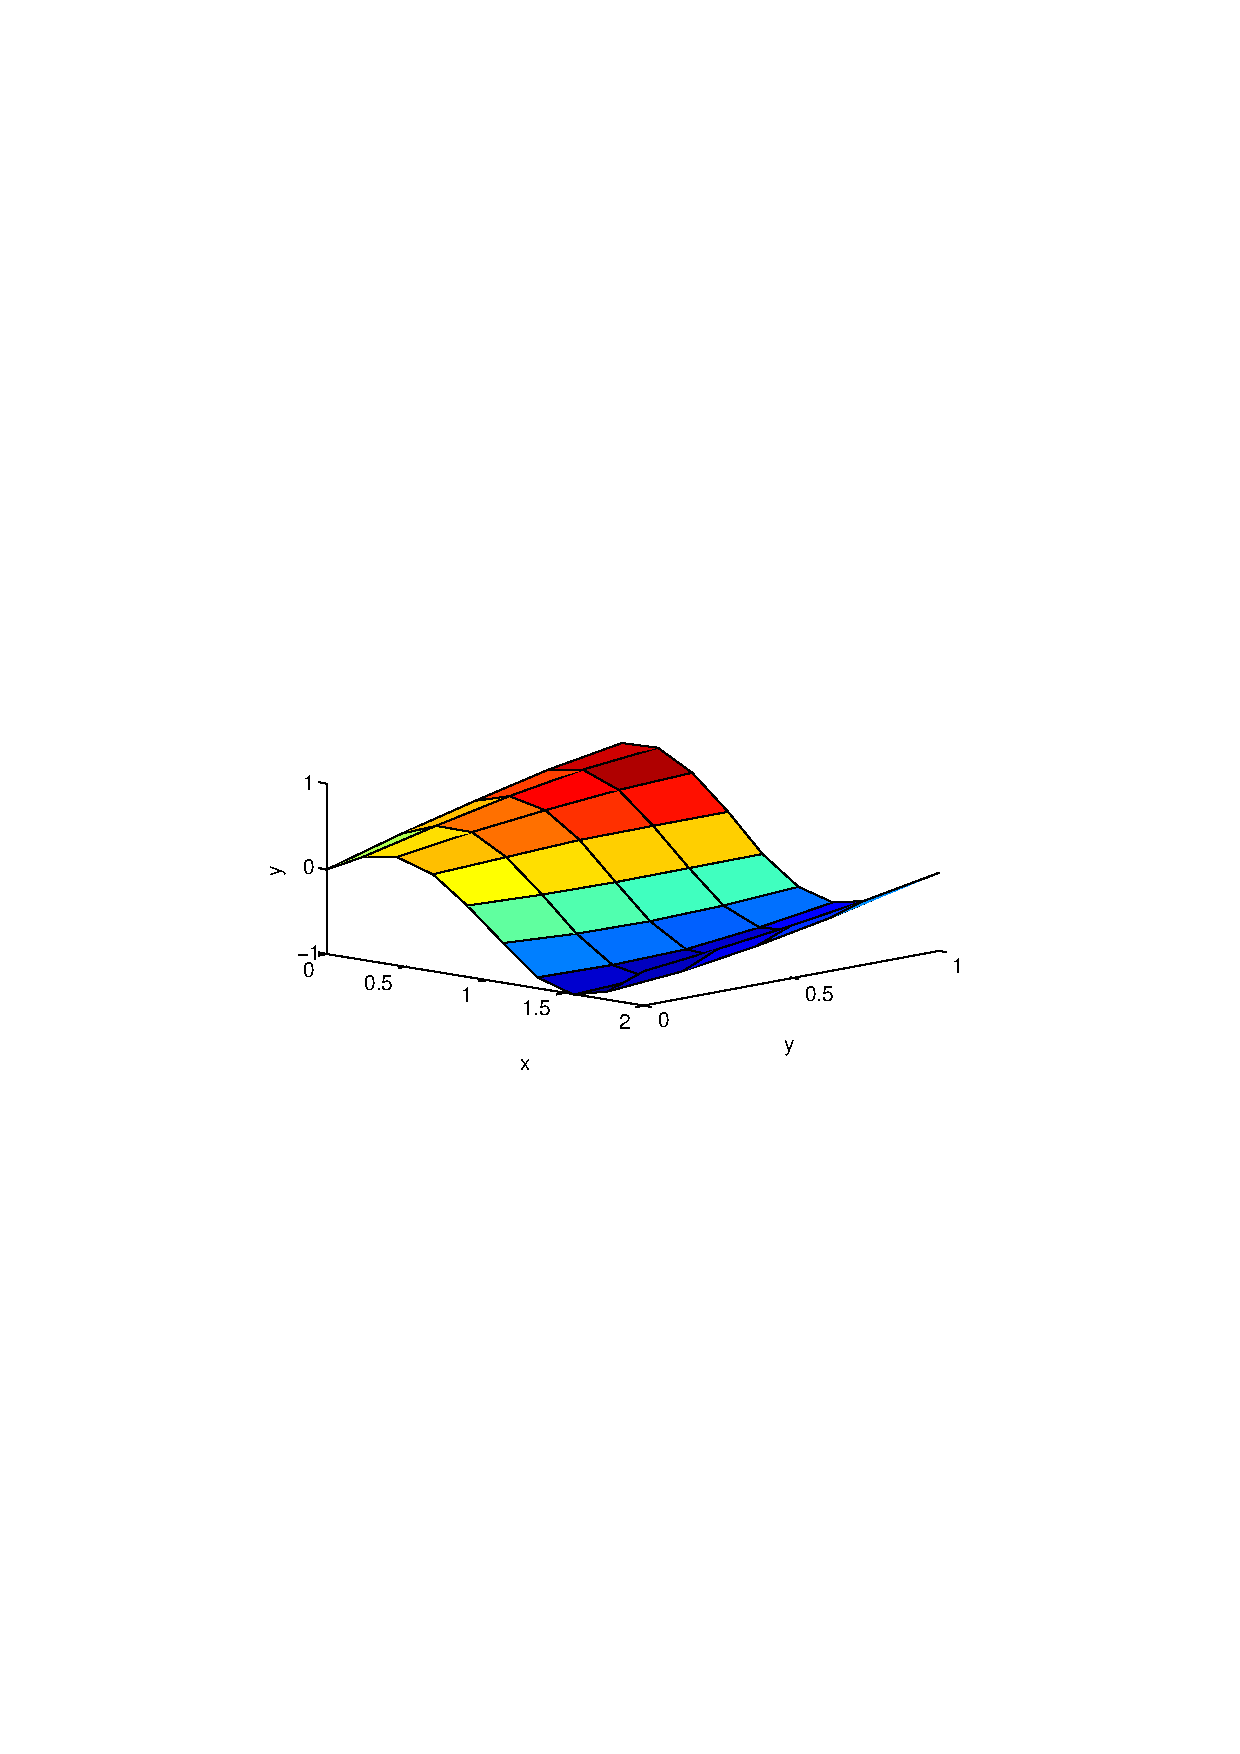
\includegraphics[width=0.45\linewidth, trim=3cm 11cm 3cm 11cm]{figure/X.pdf}
% 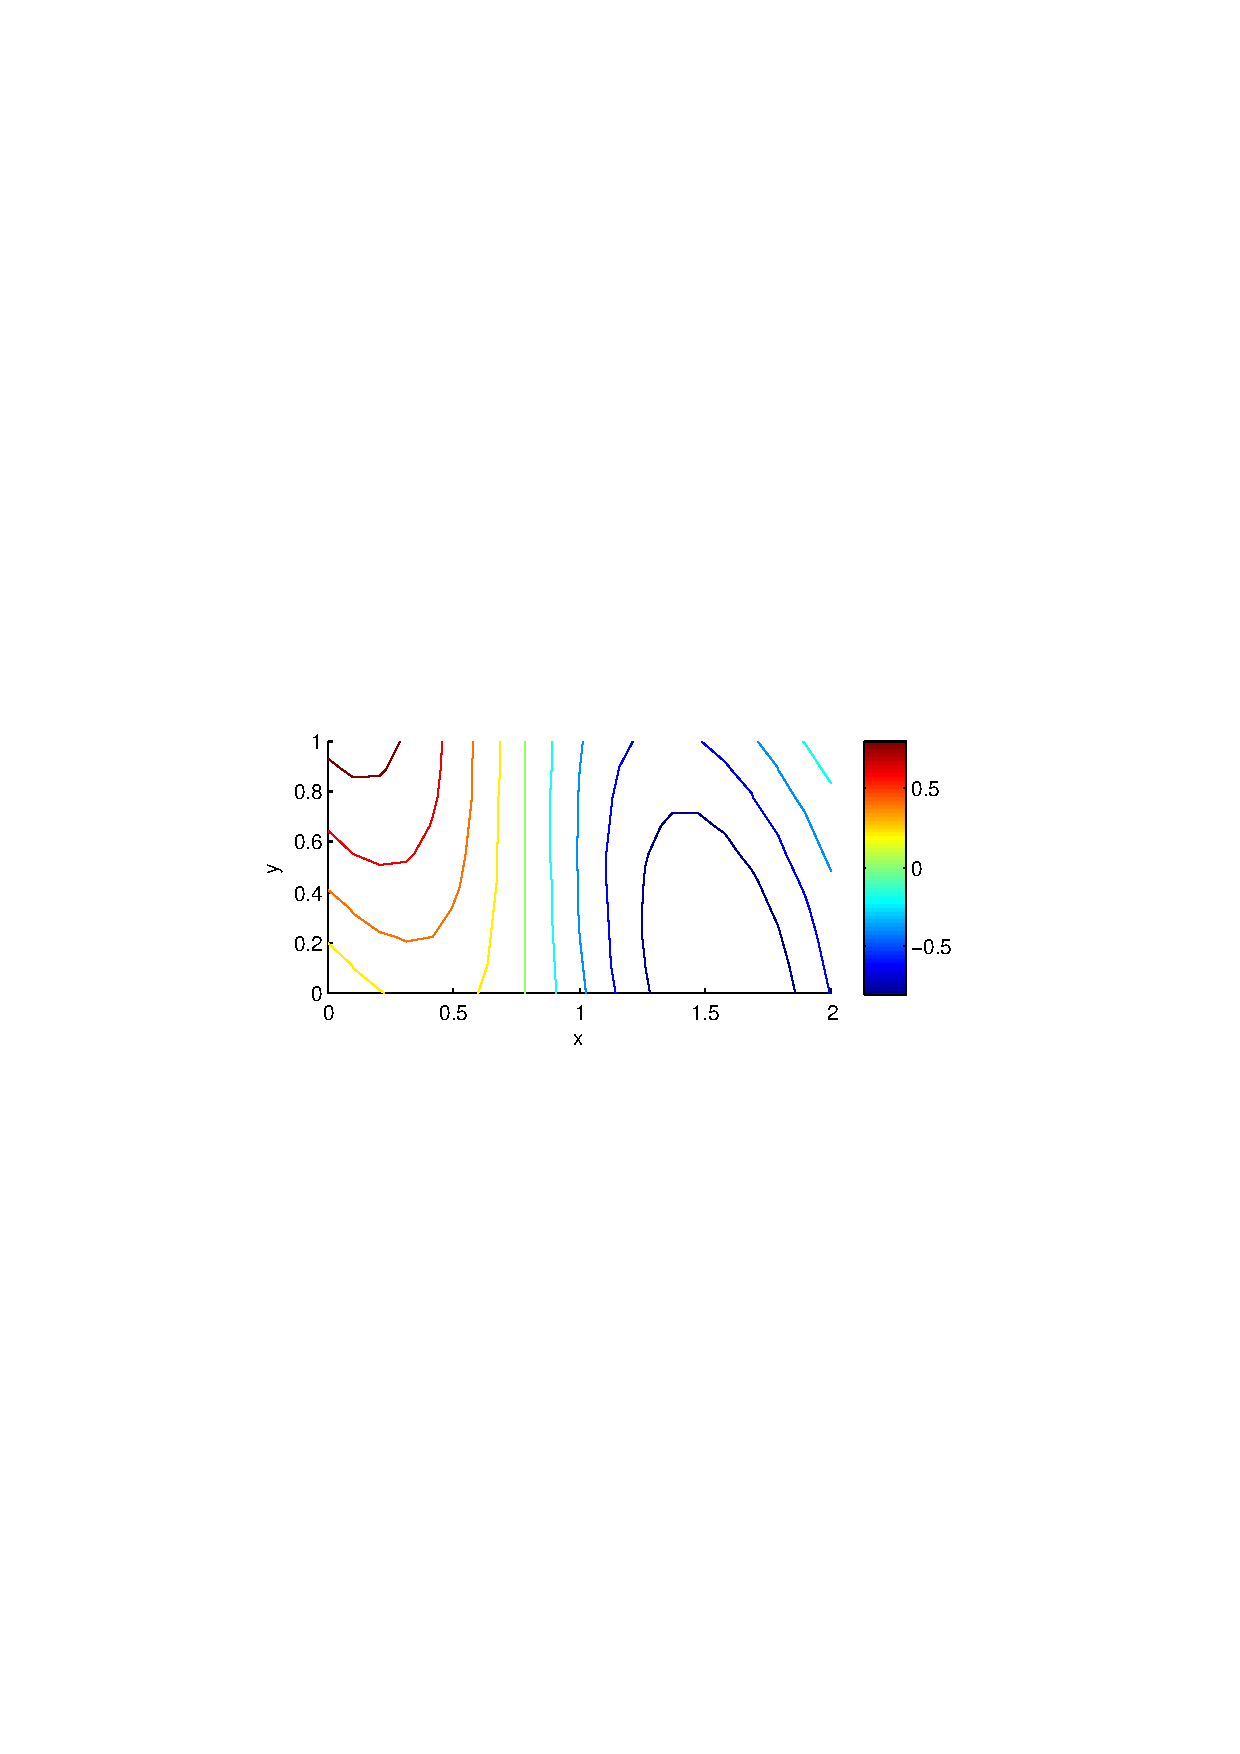
\includegraphics[width=0.45\linewidth, trim=3cm 11cm 3cm 11cm]{figure/Y.pdf}
% \caption{Surface and contour plots showing the two dimensional function $z(x,y)=\sin(x+y)\cos(2x)$.}
% \end{figure}

% \section{Equation}
% \begin{equation}
% f(t)=\left\{ \begin{array}{ll}
% 1,~~~~ & t< 1 \\
% t^2 & t\geq 1
% \end{array}\right.
% \end{equation}

% \section{Table}
% \begin{table}[H]
% \centering
% \caption{Values of $f(t)$ for $t=0,1,\dots 5$.}
% \begin{tabular}{l|llllll} \hline\hline
% $t$ & 0 & 1 & 2 & 3 & 4 & 5 \\ \hline
% $f(t)$ & 1 & 1 & 4 & 9 & 16 & 25 \\ \hline\hline
% \end{tabular}
% \end{table}

% \section{Chemical structure}
% \begin{center}
% \chemfig{X*5(-E-T-A-L-)}
% \end{center}

% \section{List}
% \begin{enumerate}
%   \item The first item
%   \begin{enumerate}
%     \item Nested item 1
%     \item Nested item 2
%   \end{enumerate}
%   \item The second item
%   \item The third item 
%   \item \dots
% \end{enumerate}

% \section{Source code listing}
% %\lstset{language=Matlab}
% \begin{lstlisting}[frame=single]
% % Generate x- and y-nodes
% x=linspace(0,1); y=linspace(0,1);

% % Calculate z=f(x,y)
% for i=1:length(x)
%  for j=1:length(y)
%   z(i,j)=x(i)+2*y(j);
%  end
% end
% \end{lstlisting}

% \section{To-do note}
% The \texttt{todo} package enables to-do notes to be added in the page margin. This can be a very convenient way of making notes in the document during the process of writing. All notes can be hidden by using the option \emph{disable} when loading the package in the settings. \todo{Example of a to-do note.}

